% Paper draft for the CVsports workshop at CVPR 2027 (xg-vendor 17). See README.md for the build.
% Every number is \val{id} from numbers.tex, generated and checked by scripts/check_vendor_paper.py.
\documentclass[10pt,twocolumn,letterpaper]{article}

\usepackage[review]{cvpr}      % review version: anonymous, line numbers; [final] for the camera-ready

\usepackage{xr-hyper}
\externaldocument[S-]{supp}
\definecolor{cvprblue}{rgb}{0.21,0.49,0.74}
\usepackage[pagebackref,breaklinks,colorlinks,allcolors=cvprblue]{hyperref}
\usepackage{multirow}
\usepackage{tabularx}

% Generated by scripts/check_vendor_paper.py --write from claims.toml; do not edit.
% \val{id} prints the number of claim id; an unknown id stops the LaTeX run.
\providecommand{\defval}[2]{\expandafter\def\csname xgv:#1\endcsname{#2}}
\providecommand{\val}{}
\DeclareRobustCommand{\val}[1]{\ifcsname xgv:#1\endcsname\csname xgv:#1\endcsname\else\PackageError{numbers}{No number with id #1}{}\fi}
\defval{pg.code_files}{32}
\defval{run.gate_thr}{0.005}
\defval{run.prereg_sha}{312e4e4a3282}
\defval{pg.nf_matches}{86}
\defval{pg.recovered_pen}{7}
\defval{pg.ci95}{95\%}
\defval{pg.corner_margin}{0.021}
\defval{pg.near}{0.02}
\defval{run.delta}{0.005}
\defval{run.n_boot}{5,000}
\defval{pg.alpha}{5\%}
\defval{pg.ci90}{90\%}
\defval{pg.bonf}{2.5\%}
\defval{pa.p_train}{1,478}
\defval{pa.p_valid}{639}
\defval{pa.p_test}{637}
\defval{pa.secondary}{797}
\defval{pa.recovered}{50}
\defval{rd.cut}{209}
\defval{pa.sb_unpaired}{875}
\defval{pa.mispairs}{26}
\defval{pa.mispair_s}{10 s}
\defval{ti.unpaired}{285}
\defval{ti.r_shot}{36}
\defval{pa.no_sb_10s}{249}
\defval{pa.window}{2.5 s}
\defval{ti.r_other}{176}
\defval{ti.r_dead}{52}
\defval{ti.r_none}{21}
\defval{ti.verdict}{``independent''}
\defval{ti.n_subs}{686}
\defval{ti.min_subs}{50}
\defval{ti.agree_ms}{\ensuremath{\pm}200 ms}
\defval{ti.subs_share}{13.3\%}
\defval{ti.shared}{90\%}
\defval{ti.subs_median}{1788 ms}
\defval{ti.lag}{1000 ms}
\defval{ti.shots}{96.6\%}
\defval{ti.kick}{80\%}
\defval{ti.corners}{82.1\%}
\defval{pa.paired}{2,754}
\defval{pa.matches}{135}
\defval{pa.index_shots}{3,039}
\defval{pa.sn_matches}{500}
\defval{pa.rate}{90.62\%}
\defval{pa.k0_rate}{85\%}
\defval{pa.goal_rate}{99.53\%}
\defval{pa.k0_goal}{99\%}
\defval{pa.blocked}{515/890}
\defval{pa.wayward}{47/146}
\defval{pa.dropped}{74}
\defval{co.pool_shots}{36,626}
\defval{co.pool_matches}{1,491}
\defval{co.k1_ff}{0.24607}
\defval{co.k1_vendor}{0.24732}
\defval{co.k1_gap}{\ensuremath{-}0.0012}
\defval{co.k1_margin}{0.01}
\defval{co.k1_pass}{passed}
\defval{sp.eval_train}{72}
\defval{sp.eval_valid}{31}
\defval{gc.matches}{37}
\defval{gc.pass}{passed}
\defval{gc.ll_new}{0.32655}
\defval{gc.ll_old}{0.32380}
\defval{gc.ll_diff}{\ensuremath{+}0.00275 [\ensuremath{-}0.00096, \ensuremath{+}0.00650]}
\defval{gc.tol_ll}{\ensuremath{+}0.010}
\defval{gc.auc_new}{0.79240}
\defval{gc.auc_old}{0.79884}
\defval{gc.auc_diff}{\ensuremath{-}0.00643 [\ensuremath{-}0.01721, \ensuremath{+}0.00465]}
\defval{gc.tol_auc}{\ensuremath{-}0.020}
\defval{gc.shots}{825}
\defval{sp.training}{328}
\defval{cf.s1.p.chosen}{2,754}
\defval{cf.s1.p.label}{0}
\defval{cf.s1.p.pen}{33}
\defval{cf.s1.p.fx}{0}
\defval{cf.s1.p.nf}{0}
\defval{cf.s1.p.n}{2,721}
\defval{cf.s1.p.goals}{374}
\defval{cf.s1.p.matches}{135}
\defval{cf.s1.c.chosen}{3,601}
\defval{cf.s1.c.label}{12}
\defval{cf.s1.c.pen}{40}
\defval{cf.s1.c.fx}{1}
\defval{cf.s1.c.nf}{147}
\defval{cf.s1.c.n}{3,401}
\defval{cf.s1.c.goals}{417}
\defval{cf.s1.c.matches}{135}
\defval{cf.c.p.frame_vendor}{\ensuremath{+}0.0283 [\ensuremath{+}0.0168, \ensuremath{+}0.0392]}
\defval{cf.c.c.frame_vendor}{\ensuremath{+}0.0282 [\ensuremath{+}0.0184, \ensuremath{+}0.0377]}
\defval{cf.c.p.frame_ff}{\ensuremath{+}0.0272 [\ensuremath{+}0.0162, \ensuremath{+}0.0380]}
\defval{cf.c.c.frame_ff}{\ensuremath{+}0.0264 [\ensuremath{+}0.0167, \ensuremath{+}0.0355]}
\defval{cf.c.p.frame_da}{\ensuremath{+}0.0029 [\ensuremath{-}0.0083, \ensuremath{+}0.0137]}
\defval{cf.c.c.frame_da}{\ensuremath{-}0.0012 [\ensuremath{-}0.0105, \ensuremath{+}0.0075]}
\defval{cf.c.p.vendor_ff}{\ensuremath{-}0.0010 [\ensuremath{-}0.0076, \ensuremath{+}0.0057]}
\defval{cf.c.c.vendor_ff}{\ensuremath{-}0.0018 [\ensuremath{-}0.0073, \ensuremath{+}0.0037]}
\defval{cf.c.p.ff_event}{\ensuremath{-}0.0059 [\ensuremath{-}0.0109, \ensuremath{-}0.0009]}
\defval{cf.c.c.ff_event}{\ensuremath{-}0.0058 [\ensuremath{-}0.0101, \ensuremath{-}0.0013]}
\defval{cf.c.p.event_da}{\ensuremath{-}0.0184 [\ensuremath{-}0.0272, \ensuremath{-}0.0101]}
\defval{cf.c.c.event_da}{\ensuremath{-}0.0219 [\ensuremath{-}0.0300, \ensuremath{-}0.0146]}
\defval{cf.c.p.da_const}{\ensuremath{-}0.0488 [\ensuremath{-}0.0608, \ensuremath{-}0.0376]}
\defval{cf.c.c.da_const}{\ensuremath{-}0.0413 [\ensuremath{-}0.0506, \ensuremath{-}0.0323]}
\defval{cf.h3.f0.angle}{0.450 [0.409, 0.489]}
\defval{cf.h3.f0.ff_def_cone}{0.367 [0.319, 0.409]}
\defval{cf.h3.f0.ge2}{0.849 [0.826, 0.871]}
\defval{cf.h3.f0.gk_depth}{0.325 [0.269, 0.377]}
\defval{cf.h3.f0.gk_off}{0.025 [0.004, 0.063]}
\defval{cf.h3.f0.gk_dist}{0.318 [0.244, 0.384]}
\defval{cf.h3.f0.opp}{0.185 [0.149, 0.218]}
\defval{cf.h3.f0.head}{0.906 [0.883, 0.927]}
\defval{cf.h3.thr.angle}{0.25}
\defval{cf.h3.thr.head}{0.70}
\defval{cf.h4.slope}{\ensuremath{+}0.545 [\ensuremath{+}0.259, \ensuremath{+}0.857]}
\defval{cf.h4.slope_200}{\ensuremath{-}0.212 [\ensuremath{-}0.822, \ensuremath{+}0.388]}
\defval{cf.h4.early}{\ensuremath{-}0.073 [\ensuremath{-}0.150, \ensuremath{+}0.007]}
\defval{cf.h4.early_200}{\ensuremath{+}0.005 [\ensuremath{-}0.072, \ensuremath{+}0.081]}
\defval{cf.h4.late}{\ensuremath{-}0.047 [\ensuremath{-}0.114, \ensuremath{+}0.020]}
\defval{cf.h4.late_200}{\ensuremath{-}0.058 [\ensuremath{-}0.128, \ensuremath{+}0.012]}
\defval{cf.h4.n}{2,347}
\defval{cf.h4.n200}{2,284}
\defval{cf.h4.off_on}{\ensuremath{+}0.025 [\ensuremath{-}0.009, \ensuremath{+}0.057]}
\defval{cf.h4.off_on_u}{\ensuremath{+}0.041 [\ensuremath{+}0.007, \ensuremath{+}0.073]}
\defval{cf.pen.p.n}{33}
\defval{cf.pen.p.goals}{22}
\defval{cf.pen.p.vp}{0.783}
\defval{cf.pen.p.vll}{0.6727}
\defval{cf.pen.p.fp}{0.697}
\defval{cf.pen.p.fll}{0.6387}
\defval{cf.pen.p.pp}{0.758}
\defval{cf.pen.p.pll}{0.6578}
\defval{cf.pen.c.n}{40}
\defval{cf.pen.c.goals}{29}
\defval{cf.pen.c.vp}{0.783}
\defval{cf.pen.c.vll}{0.5977}
\defval{cf.pen.c.fp}{0.697}
\defval{cf.pen.c.fll}{0.5900}
\defval{cf.pen.c.pp}{0.758}
\defval{cf.pen.c.pll}{0.5911}
\defval{cf.h2.p.diff}{\ensuremath{-}0.0004 [\ensuremath{-}0.0026, \ensuremath{+}0.0018]}
\defval{cf.h2.p.tost}{0.0006}
\defval{cf.h3.f0.dist}{0.711 [0.678, 0.739]}
\defval{cf.h3.f0.cone}{0.761 [0.743, 0.778]}
\defval{cf.m.p.constant}{0.4006 [0.3751, 0.4271]}
\defval{cf.a.p.constant}{0.477}
\defval{cf.m.c.constant}{0.3722}
\defval{cf.m.p.dist_angle}{0.3518 [0.3257, 0.3783]}
\defval{cf.a.p.dist_angle}{0.741}
\defval{cf.m.c.dist_angle}{0.3309}
\defval{cf.m.p.event}{0.3333 [0.3076, 0.3591]}
\defval{cf.a.p.event}{0.778}
\defval{cf.m.c.event}{0.3091}
\defval{cf.m.p.freeze_frame}{0.3275 [0.3016, 0.3538]}
\defval{cf.a.p.freeze_frame}{0.788}
\defval{cf.m.c.freeze_frame}{0.3033}
\defval{cf.m.p.vendor}{0.3264 [0.3016, 0.3515]}
\defval{cf.a.p.vendor}{0.792}
\defval{cf.m.c.vendor}{0.3015}
\defval{cf.m.p.frame}{0.3547 [0.3298, 0.3802]}
\defval{cf.a.p.frame}{0.736}
\defval{cf.m.c.frame}{0.3297}
\defval{cf.m.p.frame_ff}{0.3271 [0.3017, 0.3538]}
\defval{cf.a.p.frame_ff}{0.789}
\defval{cf.m.c.frame_ff}{0.3028}
\defval{cf.m.p.frame_vendor}{0.3258 [0.3016, 0.3510]}
\defval{cf.a.p.frame_vendor}{0.792}
\defval{cf.m.c.frame_vendor}{0.3007}
\defval{cf.c.p.auc_frame_vendor}{\ensuremath{-}0.056 [\ensuremath{-}0.080, \ensuremath{-}0.031]}
\defval{cf.r.p.vendor}{\ensuremath{-}0.0328 [\ensuremath{-}0.0456, \ensuremath{-}0.0205]}
\defval{cf.r.p.ff}{\ensuremath{-}0.0274 [\ensuremath{-}0.0399, \ensuremath{-}0.0155]}
\defval{cf.r.p.frame}{\ensuremath{-}0.0041 [\ensuremath{-}0.0182, \ensuremath{+}0.0092]}
\defval{cf.h2.p.ci90}{[\ensuremath{-}0.0022, \ensuremath{+}0.0015]}
\defval{cf.h2.p.sup}{0.5274}
\defval{cf.h2.p.margin}{0.0022}
\defval{cf.h2.c.diff}{\ensuremath{-}0.0005 [\ensuremath{-}0.0025, \ensuremath{+}0.0012]}
\defval{cf.h2.c.ci90}{[\ensuremath{-}0.0021, \ensuremath{+}0.0010]}
\defval{cf.h2.c.tost}{0.0000}
\defval{cf.h2.c.sup}{0.4030}
\defval{cf.h2.c.margin}{0.0021}
\defval{cf.fv.p.diff}{\ensuremath{-}0.0007 [\ensuremath{-}0.0034, \ensuremath{+}0.0020]}
\defval{cf.fv.p.ci90}{[\ensuremath{-}0.0028, \ensuremath{+}0.0016]}
\defval{cf.fv.p.tost}{0.0042}
\defval{cf.fv.p.sup}{0.4384}
\defval{cf.fv.p.margin}{0.0029}
\defval{cf.fv.c.diff}{\ensuremath{-}0.0008 [\ensuremath{-}0.0032, \ensuremath{+}0.0012]}
\defval{cf.fv.c.ci90}{[\ensuremath{-}0.0027, \ensuremath{+}0.0010]}
\defval{cf.fv.c.tost}{0.0018}
\defval{cf.fv.c.sup}{0.3158}
\defval{cf.fv.c.margin}{0.0027}
\defval{cf.h2.p.reading}{``equivalent at $\delta$: the frame adds no more than $\delta$''}
\defval{cf.h2.p.point}{\ensuremath{-}0.0004}
\defval{cf.h2.p.ci95}{[\ensuremath{-}0.0026, \ensuremath{+}0.0018]}
\defval{cf.h2.c.reading}{equivalent at $\delta$: the frame adds no more than $\delta$}
\defval{cf.h2.p.sd}{0.00111}
\defval{cf.ctl.f0}{\ensuremath{-}0.0006}
\defval{cf.ctl.f1}{\ensuremath{+}0.0005}
\defval{cf.ctl.dino}{\ensuremath{-}0.0002}
\defval{cf.h3.n}{2,721}
\defval{cf.h3.thr.dist}{0.50}
\defval{cf.h3.f0.dist.reading}{encodes}
\defval{cf.h3.f1.dist}{0.716 [0.685, 0.743]}
\defval{cf.h3.f1.dist.reading}{encodes}
\defval{cf.h3.d.dist}{0.684 [0.656, 0.711]}
\defval{cf.d.f0.dist}{\ensuremath{+}0.027 [\ensuremath{+}0.011, \ensuremath{+}0.042]}
\defval{cf.h3.thr.cone}{0.70}
\defval{cf.h3.f0.cone.reading}{encodes}
\defval{cf.h3.f1.cone}{0.758 [0.741, 0.775]}
\defval{cf.h3.f1.cone.reading}{encodes}
\defval{cf.h3.d.cone}{0.735 [0.716, 0.754]}
\defval{cf.d.f0.cone}{\ensuremath{+}0.025 [\ensuremath{+}0.013, \ensuremath{+}0.038]}
\defval{cf.d.f1.dist}{\ensuremath{+}0.032 [\ensuremath{+}0.018, \ensuremath{+}0.046]}
\defval{cf.d.f1.cone}{\ensuremath{+}0.023 [\ensuremath{+}0.010, \ensuremath{+}0.035]}
\defval{cf.h4.on}{1,079}
\defval{cf.h4.main}{\ensuremath{+}0.056 [\ensuremath{+}0.004, \ensuremath{+}0.108]}
\defval{cf.h4.main_u}{\ensuremath{-}0.034 [\ensuremath{-}0.107, \ensuremath{+}0.036]}
\defval{cf.h4.off_mean}{\ensuremath{+}0.057 [\ensuremath{+}0.041, \ensuremath{+}0.073]}
\defval{dv.target}{0.80}
\defval{dv.pow002}{0.284}
\defval{dv.pow003}{0.509}
\defval{dv.pow005}{0.849}
\defval{dv.margins}{0.002, 0.003 and 0.005}
\defval{dv.chosen}{0.005}
\defval{dv.m002}{0.002}
\defval{dv.pow_null}{0.949}
\defval{dv.h2}{\ensuremath{-}0.0007 [\ensuremath{-}0.0031, \ensuremath{+}0.0016]}
\defval{dv.h2_margin}{0.0028}
\defval{dv.frame_vendor}{\ensuremath{+}0.0274 [\ensuremath{+}0.0159, \ensuremath{+}0.0382]}
\defval{dv.n_sims}{1,000}
\defval{dv.sd_dev}{0.00119}
\defval{dv.sd_null}{0.00042}
\defval{dv.rc.sims}{80}
\defval{dv.rc.dev_refit}{0.00120}
\defval{dv.rc.null_refit}{0.00072}
\defval{dv.rc.null_shift}{\ensuremath{+}0.00025}
\defval{dv.rc.dev_fixed}{0.00103}
\defval{dv.rc.null_fixed}{0.00036}
\defval{dv.probe_n}{489}
\defval{dv.probe_dist}{\ensuremath{+}0.071 [\ensuremath{+}0.025, \ensuremath{+}0.122]}

\newcommand{\sbattr}{Data: StatsBomb.}   % required on every table and figure built from StatsBomb data
% Review version: no link (CVPR forbids links that identify the authors). Camera-ready: the public repository URL.
\newcommand{\codelink}{[anonymised repository link withheld for review; released on acceptance]}
\newcommand{\Hone}{H1\xspace}\newcommand{\Htwo}{H2\xspace}\newcommand{\Hthree}{H3\xspace}\newcommand{\Hfour}{H4\xspace}

\def\paperID{*****}
\def\confName{CVPR}
\def\confYear{2027}

\title{What Does One Broadcast Frame Add to Expected Goals?\\A Pre-registered Comparison with Positional and Vendor xG}

\author{Anonymous CVsports submission}

\begin{document}
\maketitle

\begin{abstract}
Expected goals (xG) is the probability that a shot becomes a goal. Data vendors estimate it from event and positional
data that human annotators collect; a model that reads one broadcast frame needs neither. We ask how frame-based xG
compares with vendor xG and with positional xG on the same shots, and what the frame model encodes. We pair
\val{pa.paired} SoccerNet shots in \val{pa.matches} matches one to one with StatsBomb open-data shots, retrain our
frame model (a DINOv2-L backbone fine-tuned on single frames) without these matches, freeze a gradient-boosted
positional comparator that ties the vendor,
and fix hypotheses, margins, readings and analysis code by hash before any outcome label is joined. The analysis then
ran once. Our confirmatory results: adding the frame to the positional comparator changes log-loss by \val{cf.h2.p.diff},
which is equivalent at the pre-registered margin $\delta = \val{run.delta}$ (TOST $p = \val{cf.h2.p.tost}$): the frame
adds no more than $\delta$. Linear probes read shot distance ($R^2$ \val{cf.h3.f0.dist}) and the presence of a
defender in the shooting cone (AUC \val{cf.h3.f0.cone}) from the frame embedding above pre-registered thresholds, and
better than from the frozen backbone (a secondary comparison, not corrected for multiplicity). Alone, the frame is worse than vendor xG by \val{cf.c.p.frame_vendor} log-loss
(descriptive). The frame model encodes shot geometry, but within $\delta$ it holds no information about the goal that
the positional data lack. We release identifiers, predictions and code, but no vendor data.
\end{abstract}

\section{Introduction}
\label{sec:intro}

Expected goals (xG) models give each shot a probability of becoming a goal. They are a widely used measure of chance
quality in football analytics~\cite{rathke2017examination,lucey2015quality,decroos2019actions}. Commercial xG comes
from data vendors. Their annotators record every shot with its location, body part, the play that led to it and, for
some data products, a \emph{freeze frame}: the positions of the players visible at the moment of the shot. A model
that reads the broadcast video could produce xG for any televised match without annotation, and it might see things
that annotators do not record, such as the shooter's posture and balance.

A frame model that is evaluated only against other frame models leaves three questions open.
How does xG from one broadcast frame compare with vendor xG and with xG from positional data on the same shots? Does
the frame add information about the goal beyond what positional data hold? And what does the frame model encode?
These questions are hard to answer cleanly. Shot outcomes are noisy, a few thousand shots resolve only differences of a
few thousandths of log-loss, and every analysis choice (population, recalibration, margin, which contrasts count) can
move such small differences. We therefore ran the comparison as a pre-registered study~\cite{nosek2018preregistration}:
all choices were fixed and hashed before any outcome label was joined to the new predictions, and the analysis ran
once.

Our contributions:
\begin{itemize}[leftmargin=*,itemsep=1pt,topsep=2pt]
  \item A one-to-one pairing of SoccerNet-v2 shots~\cite{deliege2021soccernetv2} with StatsBomb open
  data~\cite{statsbomb_opendata}: \val{pa.paired} of \val{pa.index_shots} annotated shots in \val{pa.matches} matches,
  checked by a second independent implementation, with an audit of the shots each source misses (\cref{sec:data}).
  \item A pre-registered design for comparing a vision model with vendor data: a frame model retrained without the
  evaluation matches, a positional comparator that must tie the vendor before the study goes on, an equivalence margin
  chosen by a rule written before the power simulation, and decision rules and narratives fixed in
  advance (\cref{sec:method}).
  \item Confirmatory answers (\cref{sec:results}): the frame model encodes shot geometry (\Hthree), and, in a secondary
  comparison without multiplicity correction, fine-tuning makes it more linearly readable than in the frozen backbone;
  yet the frame adds no more than the margin to the positional comparator (\Htwo), and alone it is clearly worse than vendor and positional xG (\Hone, descriptive).
  \item A release of the pairing identifiers, our frame predictions and our code that contains no vendor data, so
  that anyone with access to both sources can rebuild every table (\cref{sec:availability}).
\end{itemize}

\section{Related work}
\label{sec:related}

\paragraph{Expected goals.} xG models are fitted to shot location, angle and shot context from event
data~\cite{rathke2017examination,robberechts2020data}. Tracking or positional data add the positions of defenders
and the goalkeeper~\cite{lucey2015quality,anzer2021goal}. Robberechts and Davis~\cite{robberechts2020data} studied how
much event data such models need. We compare these information levels on identical shots and add a vision rung.

\paragraph{Broadcast soccer video.} SoccerNet~\cite{giancola2018soccernet} and SoccerNet-v2~\cite{deliege2021soccernetv2}
provide broadcast video of professional matches with timestamped action annotations, including shots, and are the
standard benchmarks for action spotting. We use their shot annotations as anchors for the frame model.

\paragraph{Probing representations.} Linear probes measure what a frozen representation makes linearly
available~\cite{alain2017probes}; control tasks guard against probes that memorise~\cite{hewitt2019control}. We probe
the fine-tuned frame model and its frozen DINOv2 backbone~\cite{oquab2024dinov2} for positional quantities taken from
the vendor's freeze frames.

\paragraph{Equivalence testing and pre-registration.} Absence of a significant difference is not evidence of no
difference. The two one-sided tests (TOST) procedure~\cite{schuirmann1987tost,lakens2017equivalence} tests whether a
difference lies within a margin fixed in advance. Pre-registration fixes hypotheses and analyses before the
data that decide them are seen~\cite{nosek2018preregistration}.

\section{Data and populations}
\label{sec:data}

\paragraph{Sources.} SoccerNet-v2 annotates \val{pa.sn_matches} broadcast matches with timestamped actions. Our shot
index takes its shot annotations (\emph{shots on target}, which include blocked shots, and \emph{shots off target})
with the goal label; the annotated time is the \emph{shot anchor}, and the frame model reads the frame at the anchor
(offset 0). StatsBomb open data~\cite{statsbomb_opendata} provide events, freeze frames and the vendor's xG for each
shot. The two sources overlap in \val{pa.matches} matches: the 2015/16 season of five European leagues and the La Liga
seasons with Barcelona.

\paragraph{Pairing.} Matches are paired on Labels-v2 metadata: same competition, date within one day, exact score, and
club-name similarity with an alias list. Shots are paired per half after estimating the half's clock offset, by a
one-to-one Hungarian assignment~\cite{kuhn1955hungarian} within a \val{pa.window} window and with an ``unpaired''
option. A second implementation, written without reading the first, gave the same pairs. The pairing had to pass a kill
rule (K0) before the study went on: \val{pa.paired} of \val{pa.index_shots} index shots are paired (\val{pa.rate},
rule: at least \val{pa.k0_rate}) and the goal labels agree on \val{pa.goal_rate} of pairs (rule: at least
\val{pa.k0_goal}).

\paragraph{Populations.} The \emph{primary} population is the paired SoccerNet shots; it decides \Htwo. SoccerNet does not
annotate every shot: it has \val{pa.blocked} of StatsBomb's blocked shots and \val{pa.wayward} of its wayward ones. The
\emph{secondary} population therefore adds \val{pa.secondary} StatsBomb shots that SoccerNet never annotated and
\val{pa.recovered} of the \val{pa.dropped} SoccerNet goals without a shot annotation, recovered one to one. Their frames
were cut from re-downloaded match videos at the StatsBomb time plus the half offset. The \emph{combined} population
(primary and secondary) serves only as a pre-registered robustness check. The goal label is always SoccerNet's, the
label the frame model was trained on. Penalties are reported separately. Supplementary \cref{S-sec:audit} gives the
full audit.

\paragraph{Timing.} SoccerNet anchors and StatsBomb shot times agree closely, which could mean a shared clock. A test
written before it ran compared substitutions, which SoccerNet marks when the broadcast shows them: they agree within
\val{ti.agree_ms} in only \val{ti.subs_share} of cases, so the verdict is \val{ti.verdict}: StatsBomb time is a
separate annotation of the same broadcast, not a copy of SoccerNet's clock (Supp.~\cref{S-sec:timing}). Secondary frames, anchored on StatsBomb time, can therefore lie a few hundred
milliseconds from the contact.

\begin{table*}[t]
\centering\small
\begin{tabularx}{\linewidth}{@{}>{\raggedright\arraybackslash}p{0.27\linewidth}>{\raggedright\arraybackslash}X>{\raggedright\arraybackslash}p{0.11\linewidth}>{\raggedright\arraybackslash}p{0.13\linewidth}>{\raggedright\arraybackslash}p{0.13\linewidth}@{}}
\toprule
Information & Frame (G-combo) & Events & Positions & Vendor xG \\
\midrule
Shooter location on the pitch & indirect, from the camera view & coordinates & yes & yes \\
Body part, technique, shot type & body part usually visible, technique not always & yes & yes & yes \\
Pass before the shot (cross, through ball, cut-back) & no & yes & yes & yes \\
Pressure, first-time shot & indirect, if the opponent is in view & StatsBomb flags & yes & yes \\
Defenders and goalkeeper at the shot & only those in the camera view & no & players StatsBomb recorded & in the data; use unknown \\
Ball height at contact & no, one frame has no depth & no & no & yes, per the vendor \\
Shooter posture and balance & yes, if the camera shows them & no & no & no \\
What happens after the contact & possible if the anchor is late (\Hfour) & no, fields excluded & no & no, xG is pre-shot \\
\bottomrule
\end{tabularx}
\caption{What each source sees. ``Events'' and ``Positions'' are rungs of our positional comparator; ``Positions''
adds the freeze frame. For the vendor model we know only what StatsBomb documents. \sbattr}
\label{tab:sources}
\end{table*}

\section{Models and pre-registered analysis}
\label{sec:method}

\paragraph{Frame model (G-combo).} A DINOv2-L backbone~\cite{oquab2024dinov2} with its last four blocks fine-tuned,
an attention-pooling head and an auxiliary on-target head, trained on the goal label of the single frame at the shot
anchor, with a mask over broadcast overlays and random resized crops. Five folds grouped by home team and two seeds
give ten fold models; their logits are averaged and calibrated once by Platt scaling~\cite{platt1999probabilistic} on the training
pool. Because the archived model had trained on most study matches, we retrained it with the archived recipe on
\val{sp.training} matches outside the study. A gate test on \val{gc.matches} matches that neither model saw
(\val{gc.shots} shots) had to pass before the study went on: log-loss \val{gc.ll_new} against \val{gc.ll_old} for the
archived model, within the tolerance of \val{gc.tol_ll}. Every evaluation shot is outside the training data of every
model.

\paragraph{Positional comparator.} A histogram gradient-boosting model~\cite{friedman2001greedy,pedregosa2011sklearn}
trained once on \val{co.pool_shots} shots from \val{co.pool_matches} StatsBomb matches outside the study, with
post-contact fields excluded. Its rungs are a constant, distance and angle, event features, and event plus freeze-frame
features, which we call \emph{positions}. Kill rule K1 required the positions rung's cross-validated log-loss on that
pool to be within \val{co.k1_margin} of the vendor's: it reached \val{co.k1_ff} against the vendor's \val{co.k1_vendor}.

\paragraph{Ladder and recalibration.} Every rung, including the vendor and the frame, is recalibrated by Platt scaling
cross-fitted on five match-grouped folds of the evaluation population, shared by all rungs, so that no rung wins by
calibration alone. Stacks (frame + positions, frame + vendor) are logistic regressions on two logits, cross-fitted on
the same folds. Inference uses a match-clustered bootstrap~\cite{field2007bootstrapping} with \val{run.n_boot} draws,
the same draws for every contrast; recalibration and stacks are refitted in every draw. We report log-loss as the
primary metric~\cite{gneiting2007scoring} and AUC.

\paragraph{Hypotheses.} \Hone (descriptive) is the information ladder: every rung on the same shots. \Htwo
(confirmatory) is $\Delta = \mathrm{LL}(\text{frame + positions}) - \mathrm{LL}(\text{positions})$ on the primary
population, tested by TOST at $\delta = \val{run.delta}$ with \val{pg.alpha} per side, i.e.\ equivalence when the
\val{pg.ci90} interval lies inside $(-\delta, \delta)$, with a one-sided superiority test beside it. $\delta$ is the
smallest of three candidate margins with sufficient simulated power, by a rule written before the simulation
(Supp.~\cref{S-sec:dev}). A fixed table maps the two tests and the sign of the interval to a reading; the reading
``equivalent at $\delta$: the frame adds no more than $\delta$'' requires equivalence, no superiority and a
\val{pg.ci95} lower bound not above zero. \Hthree (confirmatory) asks what the frame encodes: dual ridge probes~\cite{hoerl1970ridge} from
the frame embedding (offset 0) to quantities computed from the StatsBomb freeze frame and shot location, with nested
match-grouped cross-validation and standardisation fitted inside the training folds. The fold-0 model decides; the
fold-1 model is a sensitivity check; frozen DINOv2-L with the backbone's weights is the reference. Two targets are
confirmatory, distance to goal ($R^2$) and at least one defender in the shooting cone (AUC), each decided by the lower
bound of its \val{pg.ci95} interval against a threshold, i.e.\ a one-sided test at \val{pg.bonf} (Bonferroni~\cite{dunn1961multiple}).
Eight further targets are descriptive. A probe on row-shuffled distance is a hard negative-control gate: its $R^2$ must
not exceed \val{run.gate_thr} for an encoder's readings to count. \Hfour (descriptive) is a leakage diagnostic: does
the frame read the ball's direction after the contact? It regresses the frame--vendor logit gap on SoccerNet's
on-target flag with fixed controls (vendor logit, body part, shot type) and contrasts the frame logit at offset 0
with the one at $-400$\,ms.

\paragraph{Protocol.} The pre-registration fixed hypotheses, populations, labels, $\delta$, recalibration, bootstrap,
probe thresholds, table shells and, for each confirmatory hypothesis, both narratives. It pinned by SHA-256 the
analysis code (\val{pg.code_files} files), the label-free evaluation table, the split plan, the comparator predictions
and two dry runs on permuted labels. A script refused to join labels unless all hashes matched; labels were joined once,
after the pre-registration was committed and approved, and the analysis ran once without deviation.
Supplementary \cref{S-sec:prereg} gives the details.

\section{Confirmatory results}
\label{sec:results}

The primary population has \val{cf.s1.p.n} non-penalty shots with \val{cf.s1.p.goals} goals in
\val{cf.s1.p.matches} matches; the combined population has \val{cf.s1.c.n}. Differences are A $-$ B in log-loss, so a
negative value favours A. Intervals are \val{pg.ci95} match-bootstrap percentile intervals.

\begin{figure*}[t]
\centering
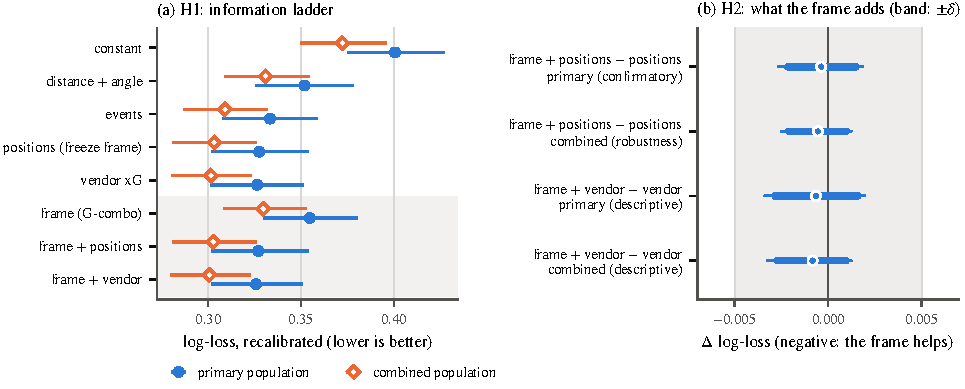
\includegraphics[width=\linewidth]{figures/fig_ladder.pdf}
\caption{Confirmatory run. (a) \Hone, descriptive: recalibrated log-loss of every rung with \val{pg.ci95} intervals; the shaded
rows use the frame. (b) \Htwo: differences with \val{pg.ci95} (thin) and \val{pg.ci90} (thick) intervals; the band is the pre-registered
margin $\pm\delta$. Equivalence holds when the \val{pg.ci90} interval lies inside the band. Combined-population frames outside
the primary population are anchored at StatsBomb time plus the half offset. \sbattr}
\label{fig:ladder}
\end{figure*}

\subsection{\Hone: information ladder (descriptive)}
\label{sec:h1}

\begin{table}[t]
\centering\small
\setlength{\tabcolsep}{4pt}
\begin{tabular}{@{}lccc@{}}
\toprule
 & \multicolumn{2}{c}{Primary} & Combined \\
\cmidrule(lr){2-3}\cmidrule(lr){4-4}
Rung & Log-loss [\val{pg.ci95}] & AUC & Log-loss \\
\midrule
Constant & \val{cf.m.p.constant} & \val{cf.a.p.constant} & \val{cf.m.c.constant} \\
Distance + angle & \val{cf.m.p.dist_angle} & \val{cf.a.p.dist_angle} & \val{cf.m.c.dist_angle} \\
Events & \val{cf.m.p.event} & \val{cf.a.p.event} & \val{cf.m.c.event} \\
Positions & \val{cf.m.p.freeze_frame} & \val{cf.a.p.freeze_frame} & \val{cf.m.c.freeze_frame} \\
Vendor xG & \val{cf.m.p.vendor} & \val{cf.a.p.vendor} & \val{cf.m.c.vendor} \\
Frame & \val{cf.m.p.frame} & \val{cf.a.p.frame} & \val{cf.m.c.frame} \\
Frame + positions & \val{cf.m.p.frame_ff} & \val{cf.a.p.frame_ff} & \val{cf.m.c.frame_ff} \\
Frame + vendor & \val{cf.m.p.frame_vendor} & \val{cf.a.p.frame_vendor} & \val{cf.m.c.frame_vendor} \\
\bottomrule
\end{tabular}
\caption{\Hone, confirmatory run, descriptive: every rung recalibrated on the same shots. The recalibrated constant has
AUC below chance because the five folds have different goal rates. \sbattr}
\label{tab:ladder}
\end{table}

\Cref{fig:ladder}a and \cref{tab:ladder} show the ladder. In both populations, the intervals of each step up the
positional ladder lie entirely below zero: distance and angle against the constant \val{cf.c.p.da_const}, events
against distance and angle \val{cf.c.p.event_da}, and positions against events \val{cf.c.p.ff_event} (primary). The
vendor and our positions rung are close: vendor $-$ positions is \val{cf.c.p.vendor_ff}, an interval that includes
zero. The frame alone is worse than both: frame $-$ vendor is \val{cf.c.p.frame_vendor} and frame $-$ positions is
\val{cf.c.p.frame_ff}, intervals entirely above zero (combined: \val{cf.c.c.frame_vendor} and \val{cf.c.c.frame_ff}).
In AUC, frame $-$ vendor is \val{cf.c.p.auc_frame_vendor}. Frame $-$ distance and angle is
\val{cf.c.p.frame_da}, an interval that includes zero.

Without recalibration, the models trained on StatsBomb data under-predict goals on the primary population: mean
probability minus goal rate is \val{cf.r.p.vendor} for the vendor and \val{cf.r.p.ff} for positions, against
\val{cf.r.p.frame} for the frame, which was trained on SoccerNet labels. SoccerNet omits many blocked and wayward
shots, so its shots have a higher goal rate than StatsBomb's.

\subsection{\Htwo: does the frame add to positions?}

\begin{table*}[t]
\centering\footnotesize
\setlength{\tabcolsep}{3pt}
\begin{tabular}{@{}llllllll@{}}
\toprule
Contrast & Population & Role & $\Delta$ [\val{pg.ci95}] & $\Delta$, \val{pg.ci90} & $p$ TOST & $p$ superior. & Smallest margin \\
\midrule
Frame + positions $-$ positions & primary & confirmatory & \val{cf.h2.p.diff} & \val{cf.h2.p.ci90} & \val{cf.h2.p.tost} & \val{cf.h2.p.sup} & \val{cf.h2.p.margin} \\
Frame + positions $-$ positions & combined & robustness & \val{cf.h2.c.diff} & \val{cf.h2.c.ci90} & \val{cf.h2.c.tost} & \val{cf.h2.c.sup} & \val{cf.h2.c.margin} \\
Frame + vendor $-$ vendor & primary & descriptive & \val{cf.fv.p.diff} & \val{cf.fv.p.ci90} & \val{cf.fv.p.tost} & \val{cf.fv.p.sup} & \val{cf.fv.p.margin} \\
Frame + vendor $-$ vendor & combined & descriptive & \val{cf.fv.c.diff} & \val{cf.fv.c.ci90} & \val{cf.fv.c.tost} & \val{cf.fv.c.sup} & \val{cf.fv.c.margin} \\
\bottomrule
\end{tabular}
\caption{\Htwo, confirmatory run: log-loss differences, TOST at $\delta = \val{run.delta}$, one-sided superiority test,
and the smallest margin at which equivalence holds. All four rows read ``equivalent at $\delta$''. Combined-population
frames outside the primary population are anchored at StatsBomb time plus the half offset. \sbattr}
\label{tab:h2}
\end{table*}

On the primary population, equivalence holds, superiority does not, and the \val{pg.ci95} lower bound is not above zero
(\cref{tab:h2}, \cref{fig:ladder}b). The pre-registered rule therefore gives the reading
\val{cf.h2.p.reading}, and the pre-registered narrative applies, with only the numbers filled in:

\begin{quote}\small
On \val{cf.s1.p.n} paired shots in \val{cf.s1.p.matches} matches, adding one broadcast frame to the positional model
changed log-loss by $\Delta = \val{cf.h2.p.point}$ (\val{pg.ci95} \val{cf.h2.p.ci95}). The equivalence test excluded a gain or a
loss larger than $\delta = \val{run.delta}$ ($p_\text{TOST} = \val{cf.h2.p.tost}$). The frame carries no information
about the chance of a goal beyond what the StatsBomb events and freeze frame contain, within $\delta$. At the same
time, the frame alone is clearly weaker than positions. The simplest explanation: what the frame sees (the positions
of shooter, defenders and goalkeeper) the vendor records more precisely, and what the vendor does not record, one
frame does not show. The smallest equivalence margin is \val{cf.h2.p.margin}, so the claim of no gain has this
precision and no more. The combined population gave: \val{cf.h2.c.reading}.
\end{quote}

The readings of both populations agree. The chosen bootstrap refits recalibration and stacks in every draw; its SD of
the primary \Htwo difference is \val{cf.h2.p.sd}. Under a true effect near zero this bootstrap is too wide
(Supp.~\cref{S-sec:dev}), which makes equivalence harder to show and the superiority test conservative.

\subsection{\Hthree: what the frame encodes}

\paragraph{Negative control.} The probe on row-shuffled distance gave $R^2$ \val{cf.ctl.f0} for the fold-0 model,
\val{cf.ctl.f1} for fold 1 and \val{cf.ctl.dino} for DINOv2, all at most \val{run.gate_thr}. The gate passed for all
three encoders, so every reading counts. The probes use \val{cf.h3.n} primary non-penalty shots.

\begin{table*}[t]
\centering\footnotesize
\setlength{\tabcolsep}{2.5pt}
\begin{tabular}{@{}llllllll@{}}
\toprule
Target & Threshold & G-combo fold 0 & Reading & G-combo fold 1 & Reading & DINOv2 & G fold 0 $-$ DINOv2 \\
\midrule
Distance to goal, $R^2$ & \val{cf.h3.thr.dist} & \val{cf.h3.f0.dist} & \val{cf.h3.f0.dist.reading} & \val{cf.h3.f1.dist} & \val{cf.h3.f1.dist.reading} & \val{cf.h3.d.dist} & \val{cf.d.f0.dist} \\
Defender in cone, AUC & \val{cf.h3.thr.cone} & \val{cf.h3.f0.cone} & \val{cf.h3.f0.cone.reading} & \val{cf.h3.f1.cone} & \val{cf.h3.f1.cone.reading} & \val{cf.h3.d.cone} & \val{cf.d.f0.cone} \\
\bottomrule
\end{tabular}
\caption{\Hthree, confirmatory run: the two confirmatory probe targets with \val{pg.ci95} intervals. A target is encoded when
the lower bound reaches the threshold (Bonferroni, two targets). The fold-0 model decides; fold 1 is a sensitivity
check. Targets are computed from StatsBomb freeze frames and shot locations. \sbattr}
\label{tab:h3}
\end{table*}

\begin{figure*}[t]
\centering
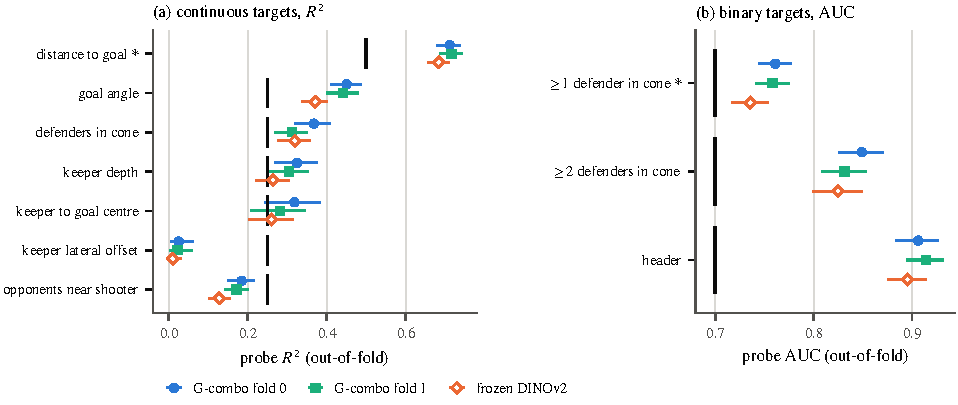
\includegraphics[width=\linewidth]{figures/fig_probes.pdf}
\caption{\Hthree, confirmatory run: linear-probe performance of the frame embedding for every target, with \val{pg.ci95}
intervals, for the deciding G-combo fold-0 model, the fold-1 sensitivity model and frozen DINOv2-L. Black ticks are the
pre-registered thresholds; * marks the two confirmatory targets, the others are descriptive. The intervals are
conditional on the fitted probes. The figure is drawn from the confirmatory probe results file; its fold-1 and DINOv2
values for the descriptive targets are not quoted in the text. \sbattr}
\label{fig:probes}
\end{figure*}

Both confirmatory targets read ``encodes'' for both fold models (\cref{tab:h3}, \cref{fig:probes}), so the
pre-registered narrative ``the frame encodes geometry'' applies:

\begin{quote}\small
From the embedding of one G-combo fold model, shot distance can be read linearly ($R^2 =$ \val{cf.h3.f0.dist},
threshold \val{cf.h3.thr.dist}), and so can the presence of a defender in the shooting cone
(AUC $=$ \val{cf.h3.f0.cone}, threshold \val{cf.h3.thr.cone}). The frame thus contains these positional quantities that
the vendor uses. Of the eight descriptive targets, the fold-0 model encodes the angle, the number of defenders in the
cone, at least two defenders in the cone, goalkeeper depth and headers; goalkeeper distance to goal is undecided; it
does not encode the goalkeeper's lateral offset or the number of opponents near the shooter. A linear probe gives only
a lower bound on what the embedding contains.
\end{quote}

\paragraph{Fine-tuned against frozen backbone.} This comparison is secondary, fixed in advance and not corrected for
multiplicity. On both confirmatory targets and for both fold models the reading is ``G $>$ DINOv2'' (fold 1:
\val{cf.d.f1.dist} for distance, \val{cf.d.f1.cone} for the cone), so the pre-registered narrative applies:

\begin{quote}\small
Fine-tuning on the goal label raised the linear readability of shot distance and of a defender in the cone by
\val{cf.d.f0.dist} ($R^2$) and \val{cf.d.f0.cone} (AUC) over the frozen backbone with the same weights. The model thus
learned to represent shot geometry rather than only use features the backbone already had. The earlier prototype
observation that fine-tuning does not help came from a probe on mixed embedding spaces of five fold models, and we do
not confirm it.
\end{quote}

Supplementary \cref{S-sec:h3more} lists the descriptive targets with both folds.

\subsection{\Hfour: leakage diagnostic (descriptive)}

Among \val{cf.h4.n} primary non-goal shots (\val{cf.h4.on} on target by SoccerNet's definition, which counts blocked
shots as on target), the frame--vendor logit gap is higher on on-target shots by \val{cf.h4.main} with the controls.
Without the controls the coefficient is \val{cf.h4.main_u}, an interval that includes zero. The frame logit rises from $-400$\,ms to the anchor by \val{cf.h4.off_mean} on
average. A positive on-target coefficient is consistent with the frame reading the ball's direction after the contact.
It is also consistent with pre-contact information that the vendor lacks, such as the shooter's balance; the data
do not separate the two. Supplementary \cref{S-sec:h4more} gives the timing-residual arm.

\section{Discussion}
\label{sec:discussion}

Fine-tuned only on goal and on-target labels, the frame model learned a representation from which shot distance and
the presence of a defender in the shooting cone can be read linearly above the pre-registered thresholds, better than
from its frozen backbone in a secondary comparison; several descriptive targets read ``encodes'' as well
(Supp.~\cref{S-sec:h3more}). It does not follow that the frame is a good source of xG next to positional data. Alone,
the frame is clearly behind the vendor and our positional comparator, and its difference from a
distance-and-angle model has an interval that includes zero. Added to positions, it adds no more than the
pre-registered margin. Both results fit the explanation written down before the run: what the frame sees (the
positions of shooter, defenders and goalkeeper) the vendor records more precisely, and what the vendor does not
record, one frame does not show. A single frame also lacks depth, and so the ball's height at contact, which the
vendor records (\cref{tab:sources}).

\section{Limitations}
\label{sec:limitations}

\begin{itemize}[leftmargin=*,itemsep=1pt,topsep=2pt]
  \item \emph{Weak gate.} The retrain was checked on \val{gc.shots} shots from \val{gc.matches} matches. The
  log-loss difference to the archived model, \val{gc.ll_diff}, has an interval that covers both no loss and a loss
  more than twice the point estimate, so the gate catches a broken retrain, not a small loss. All results concern the retrained model, which may be slightly weaker
  than the archived one.
  \item \emph{Weak \Htwo claim.} Equivalence at $\delta$ excludes only gains larger than $\delta$, and $\delta$ was
  chosen by a power rule that assumed a frame gain about twice the one the development data showed. The smallest
  equivalence margin states the actual precision.
  \item \emph{\Htwo concerns our comparator.} Positions are our freeze-frame rung, which ties the vendor in K1. The
  vendor's model has no cross-fitted version with the frame, so frame + vendor $-$ vendor is descriptive. K1 is the
  best setting of a grid and therefore slightly optimistic.
  \item \emph{Bootstrap.} The chosen bootstrap matched the sampling spread under the development truth but was too
  wide under a null truth, so the superiority test is conservative. \Hthree intervals do not refit the probes and
  omit probe-fitting variability.
  \item \emph{Descriptive \Hthree thresholds} were set with the prototype's development numbers known; the
  confirmatory thresholds predate the prototype.
  \item \emph{Population.} The primary population holds only shots SoccerNet annotated, which omits many blocked and
  wayward shots. The combined population partly repairs this, but its added frames are anchored at StatsBomb time and
  may lie a few hundred milliseconds from the contact, and it loses stoppage-time shots that the videos do not cover.
  \item \emph{Shared clubs.} Evaluation matches are outside every model's training, but their clubs play in training
  matches of other seasons, so the model may know their stadiums, kits and broadcast graphics. We did not measure
  this dependence.
  \item \emph{Ball height.} One frame does not show the ball's height at contact; the vendor knows it.
\end{itemize}

\section{Data and code availability}
\label{sec:availability}

The pre-registration, the analysis code with its hash list, the report and a number check that reads every number in
this paper back from the result files are part of the code release. The release package contains the SoccerNet game,
shot and half identifiers with their times in the half video, the StatsBomb match and event identifiers they pair with,
our pairing outcomes, the split plan of the retrain and the frame model's predictions at both offsets for every
evaluation shot. It contains no StatsBomb data (no events, locations, outcomes, freeze frames, timestamps, xG or values
computed from them) and no SoccerNet video, frames, clips, embeddings or model weights. StatsBomb's user agreement does
not allow passing its data to third parties; users fetch the open data from StatsBomb at the pinned commit and rebuild
every derived table with our code. SoccerNet video is available from its authors under their agreement. Code and
package: \codelink.

\paragraph{Attribution.} Data: StatsBomb open data (StatsBomb Services Ltd); every table and figure built from it is
marked. Video and annotations: SoccerNet-v2~\cite{deliege2021soccernetv2}.
\IfFileExists{statsbomb_logo.pdf}{\par\includegraphics[height=1.5em]{statsbomb_logo.pdf}}{}

{
    \small
    \bibliographystyle{ieeenat_fullname}
    \bibliography{refs}
}

\end{document}
